
%\vspace{-0.05in}
\section{Markov-chain Monte Carlo Estimators for Score Climbing}
\vspace{-0.05in}
\subsection{Overview of Estimation Strategies}\label{section:overview}
%
\begin{figure*}
    \centering
    \begin{subfigure}[b]{0.25\textwidth}
        \centering
        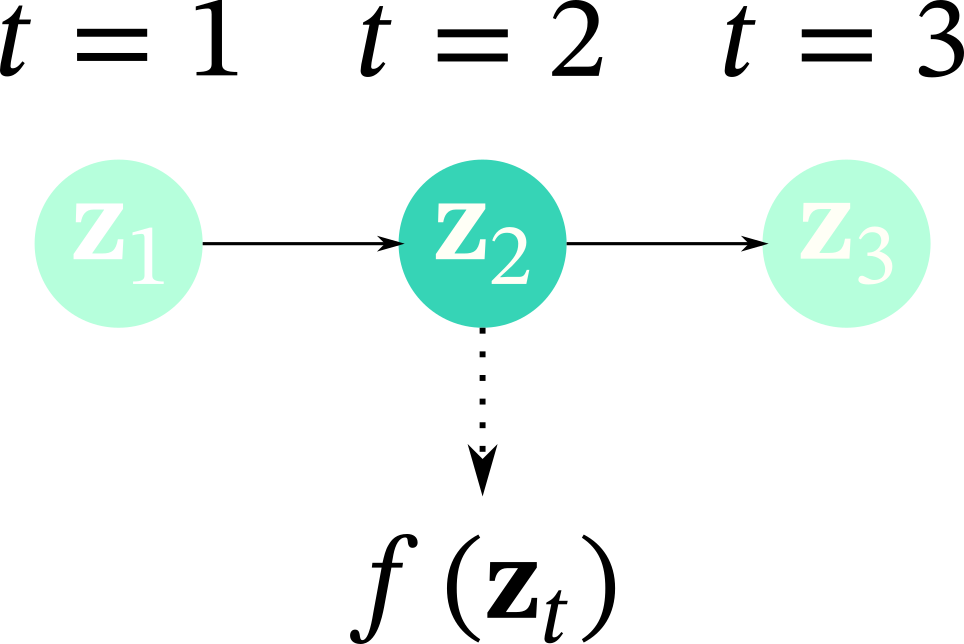
\includegraphics[scale=0.25]{figures/diagram_1.png}
        \caption{Single State Estimator}\label{fig:single}
    \end{subfigure}
    \begin{subfigure}[b]{0.35\textwidth}
        \centering
        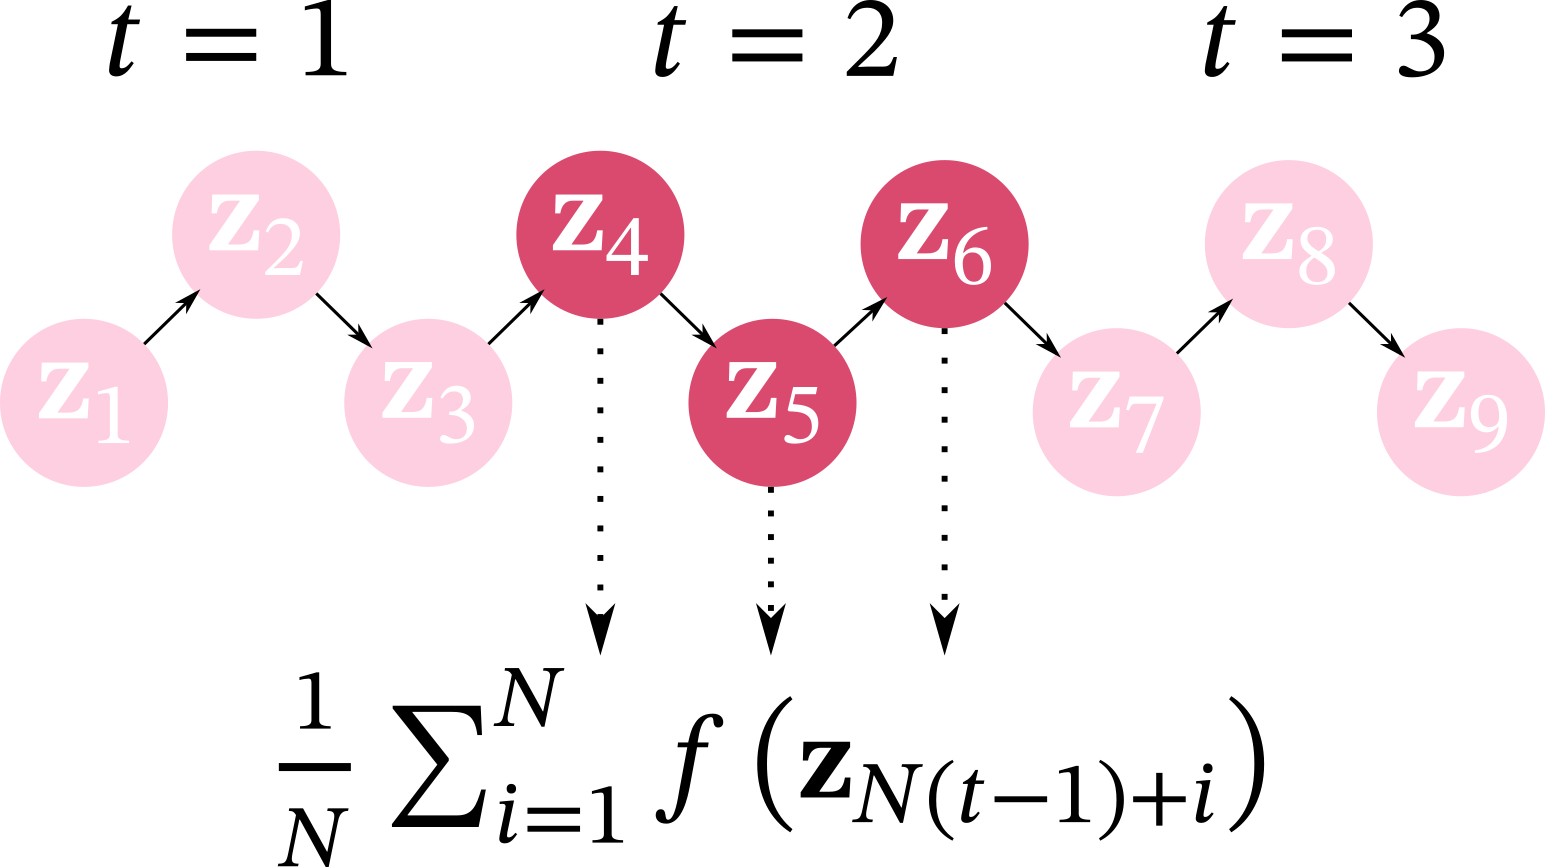
\includegraphics[scale=0.25]{figures/diagram_2.png}
        \caption{Sequential State Estimator}\label{fig:seq}
    \end{subfigure}
    \begin{subfigure}[b]{0.3\textwidth}
        \centering
        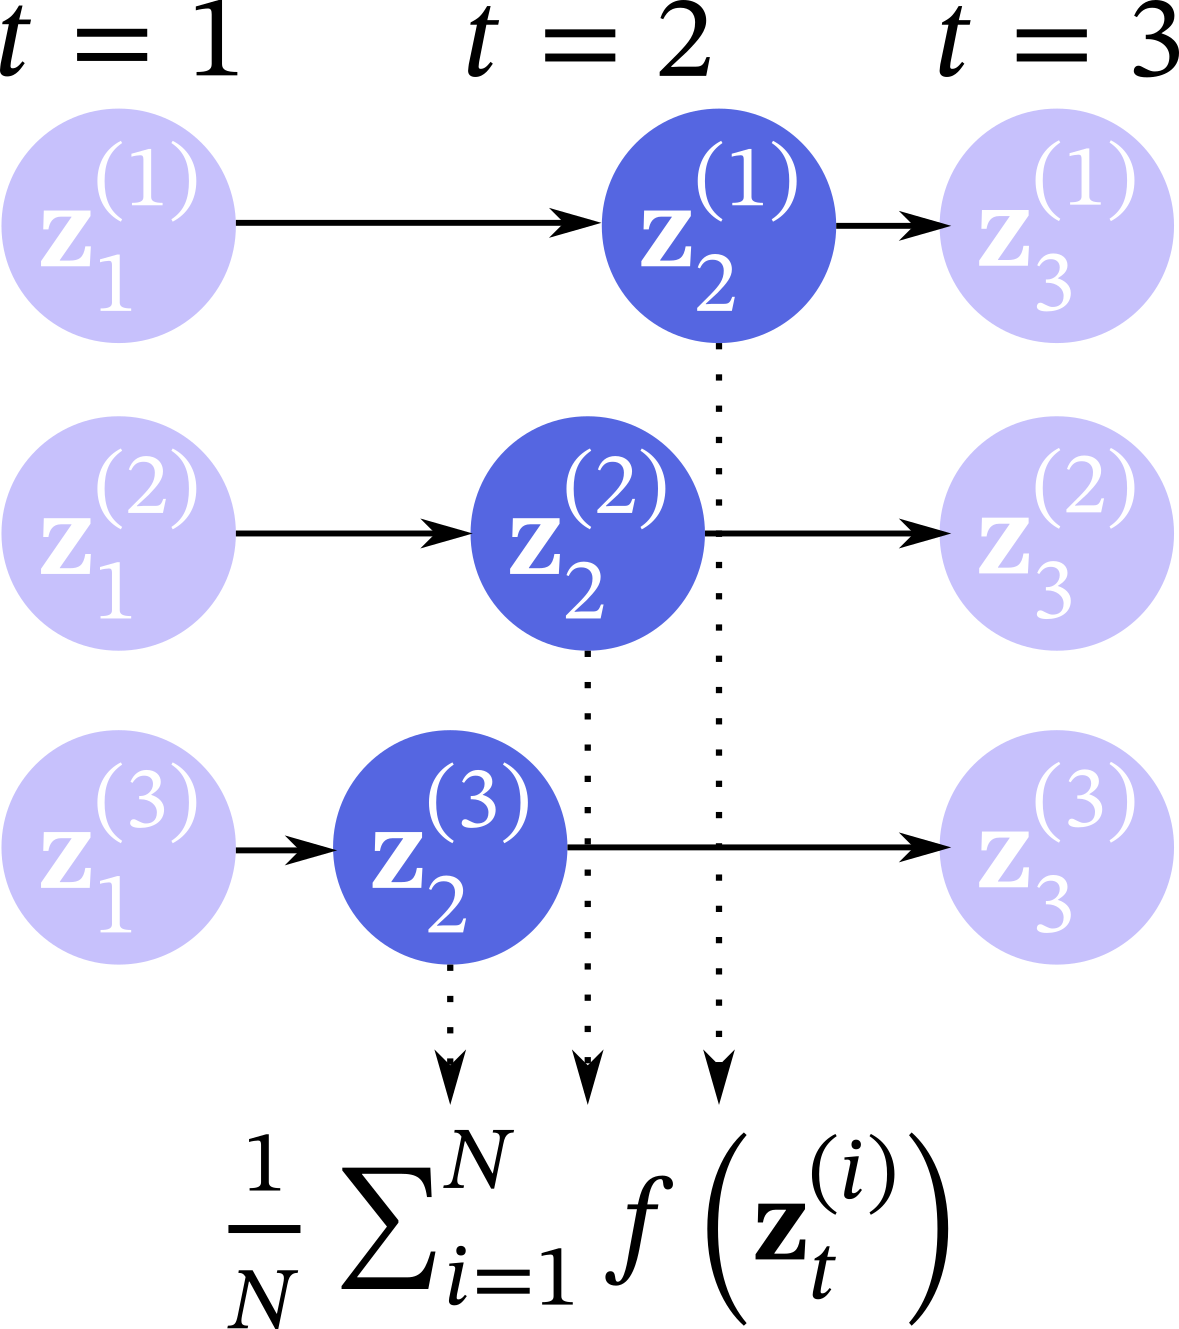
\includegraphics[scale=0.25]{figures/diagram_3.png}
        \caption{Parallel State Estimator (proposed)}\label{fig:par}
    \end{subfigure}
    \caption{Visualization of different ways of combining MCMC with stochastic approximation variational inference.
    The index \(t\) denotes the stochastic approximation iteration.
    The dark circles represent the MCMC samples used for estimating the score gradient at \(t=2\).
    }\label{fig:overview}
\end{figure*}
%

% Second version of table, with booktabs.
%\begin{table}
%\centering
\caption{Computational Costs of MCSA Schemes}\label{table:cost}
\setlength{\tabcolsep}{0.5pt}
  \begin{threeparttable}
\begin{tabular}{lccccc}\toprule
& \multicolumn{3}{c}{\footnotesize Kernel Application} & \multicolumn{2}{c}{\footnotesize Gradient Estimation} \\
\cmidrule(lr){2-4}\cmidrule(lr){5-6}
  & {\footnotesize\(p\left( \vz, \vx \right)\)}
  & {\footnotesize\(q\left(\vz; \vlambda\right)\)}
  & {\footnotesize\(q\left(\vz; \vlambda\right)\)}
  & {\footnotesize\(p\left( \vz, \vx \right)\)}
  & {\footnotesize\( q\left(\vz; \vlambda\right)\)}
  \\
  & {\footnotesize\# Eval.  }
  & {\footnotesize\# Eval.  }
  & {\footnotesize\# Samples}
  & {\footnotesize\# Grad.  }
  & {\footnotesize\# Grad.  }
%
\\\midrule
%
{\footnotesize
ELBO
}
& \(0\)
& \(0\)
& \(N\)
& \(N\)
& \(N\)
\\\arrayrulecolor{black!30}\midrule
%
{\footnotesize
MSC
}
& \(N-1\)
& \(N\)
& \(N-1\)
& \(0\)
& \(1\)\tnote{1}\;\;{\footnotesize or}\;\(N\)\tnote{2}
\\
%
{\footnotesize
JSA
}
& \(N\)
& \(N+1\)
& \(N\)
& \(0\)
& \(N\)
\\
%
{\footnotesize
\textit{pMCSA}
}
& \(N\)
& \(2 \, N\)
& \(N\)
& \(0\)
& \(N\)
\\\bottomrule
\end{tabular}
  \begin{tablenotes}
    \item[*]{\footnotesize We assume that the parameters are cached as much as possible}.
    \item[1]{\footnotesize Vanilla CIS kernel}.
    \item[2]{\footnotesize Rao-Blackwellized CIS kernel}.
  \end{tablenotes}
  \end{threeparttable}
%\end{table}

%
\vspace{-0.05in}
\paragraph{Score Climbing with MCMC}
Recently,~\citet{NEURIPS2020_b2070693} and~\citet{pmlr-v124-ou20a} proposed two similar but independent score climbing method that minimize the inclusive KL with SGD.
Both methods estimate the score function gradient by operating a Markov-chain in parallel with the VI optimization sequence.
They notably use MCMC kernels that can effectively utilize the variational approximation \(q_{\vlambda_t}(\vz)\).
Because of this, both methods are computationally more efficient than previous VI approaches~\citep{pmlr-v97-ruiz19a, pmlr-v70-hoffman17a} that used expensive MCMC kernels such as Hamiltonian Monte Carlo.

\vspace{-0.05in}
\paragraph{Single State Estimator}
In Markovian score climbing (MSC),~\citet{NEURIPS2020_b2070693} estimate the score gradient by performing an MCMC transition and estimate the score function gradient as
\vspace{-0.05in}
\begin{align*}
  &\vz_t \sim K_{\vlambda_{t-1}}\left(\vz_{t-1}, \cdot \right) \\
  &\vg_{\text{single-CIS}}(\vlambda) = \vs\,(\vz_t; \vlambda)
\end{align*}
where \(K_{\vlambda_{t-1}}\left(\vz_{t-1}, \cdot\right)\) is a MCMC kernel leaving \(p\,(\vz\mid\vx)\) invariant and \(g_{\text{single}}\left(\vlambda\right)\) denotes the score estimator.
For the MCMC kernel, they propose a new type of kernel inspired by particle MCMC~\citep{andrieu_particle_2010, andrieu_uniform_2018}, the conditional importance sampling (CIS) kernel.
Since the estimator uses \textit{a single state} created by the CIS kernel, we call it the single state estimator with the CIS kernel (single-CIS).
The CIS kernel internally uses \(N\) samples from the \(q_{\vlambda_{t-1}}(\vz)\), hence the dependence on \(\vlambda_{t-1}\).
When compared to MCMC kernels that only use a single sample from \(q_{\vlambda_{t-1}}(\vz)\), it is \(N\) times more expensive, but hopefully, statistically superior.

\vspace{-0.08in}
\paragraph{Sequential State Estimator}
On the other hand, at each SGD iteration \(t\),~\citet{pmlr-v124-ou20a} perform \(N\) sequential Markov-chain transitions and use the average of the intermediate states for estimation.
That is, for the index \(i \in \{1, \ldots, N\}\),
\vspace{-0.05in}
\begin{align*}
  &\vz_{T+i} \sim K_{\vlambda_{t-1}}^i\left(\vz_{T}, \cdot \right) \\
  &\vg_{\text{seq.-IMH}}(\vlambda) = \frac{1}{N} \sum_{i=1}^N \vs\,(\vz_{T+i}; \vlambda)
\end{align*}
where \(\vz_T\) is the last Markov-chain state of the previous SGD iteration 
\(t-1\).
\(K^{i}_{\vlambda_{t-1}}(\vz_{T}, \cdot)\) denotes the MCMC kernel sequentially applied \(i\) times.
For the MCMC kernel, they use the independent Metropolis-Hastings (IMH,~\citealt[Algorithm 25]{robert_monte_2004}~\citealt{hastings_monte_1970}) algorithm, which uses only a single sample from \(q_{\vlambda_{t-1}}(\vz)\) (notice the dependence on \(\vlambda_{t-1}\)).
Therefore, the cost of \(N\) state transitions with IMH is similar to a single transition with CIS.
Since the estimator uses sequential states, we call it the sequential state estimator with the IMH kernel (seq.-IMH)

%\subsection{The Parallel State Estimator}\label{section:overview}
\vspace{-0.08in}
\paragraph{Overview}
The single and sequential state estimators represent two different ways of using a fixed computational budget.
The former uses a single sample generated expensively, while the latter uses multiple samples generated cheaply.
Illustrations of the two schemes are provided in~\cref{fig:single,fig:seq}.

\vspace{-0.08in}
\paragraph{Parallel State Estimator}
In this work, we propose a new scheme into the mix: \textit{the parallel state estimator}.
Like the sequential state estimator, we use the cheaper IMH kernel, but instead of applying the MCMC kernel \(N\) times to a single chain, we apply the MCMC kernel a single time to \(N\) \textit{parallel Markov-chains}.
That is, for each Markov-chain indexed by \(i \in \{1, \ldots, N\}\),
%
\vspace{-0.05in}
\begin{align*}
  &\vz_{t}^{(i)} \sim K_{\vlambda_{t-1}}\big(\vz_{t-1}^{(i)}, \cdot \big) \\
  &\vg_{\text{par.-IMH}}(\vlambda) = \frac{1}{N} \sum_{i=1}^N \vs\,(\vz_{t}^{(i)}; \vlambda)
\end{align*}
%
where \(\vz_{t-1}^{(i)}\) is the state of the \(i\)th chain at the previous SGD step.
Computationally speaking, we are still applying \(K\big(\vz_{t-1}^{(i)}\big)\) \(N\) times in total, so the cost is similar to the sequential state estimator.
However, the Markov-chains are \(N\) times shorter, which, in a traditional MCMC view, might seem to result in worse statistical performance.
An illustration of the parallel state estimator is shown in~\cref{fig:par}.

\vspace{-0.05in}
\paragraph{Computational Cost}
The three schemes using the CIS kernel and the IMH kernel can have different computational costs depending on the parameter \(N\).
The computational costs of each scheme are organized in~\cref{table:cost} while detailed pseudocodes of the considered schemes are provided in the \textit{supplementary material}.
In the CIS kernel, \(N\) controls the number of internal proposals sampled from \(q_{\vlambda}(\vz)\).
In the sequential and parallel state estimators, the IMH kernel only uses a single sample from \(q_{\vlambda}(\vz)\), but applies the kernel \(N\) times.
Assuming caching is done as much as possible, the parallel state estimator needs twice the density evaluations of \(q_{\vlambda}(\vz)\) compared to other methods.
However, this added cost is minimal since the overall computational cost is dominated by  \(p(\vz,\vx)\).
When estimating the score, the single state estimator computes \(\nabla_{\vlambda} \log q_{\vlambda}(\vz)\) only once, while for the sequential and parallel state estimators compute it \(N\) times.
However,~\cite{NEURIPS2020_b2070693} also discuss a Rao-Blackwellized version of the CIS kernel, which also computes the gradient \(N\) times.
Lastly, notice that score climbing does not need to differentiate through the likelihood, unlike ELBO maximization, making it's base computational cost significantly cheaper.

\subsection{Theoretical Analysis of Bias}\label{section:theory}
\vspace{-0.05in}
\paragraph{Adaptive MCMC and Ergodicity}
For bounded functions, an upper bound on the bias of MCMC estimators can be easily derived from the convergence rates of MCMC kernels.
In the context of score climbing VI, the MCMC convergence is a subtle subject since the kernel is now \textit{adaptive} as it depends on \(\norm{\vlambda_t}\), which depends on all of the past MCMC samples.
This is clearly the type of problem adaptive MCMC algorithms have been concerned with~\citep{andrieu_ergodicity_2006}.
Fortunately, our setting crucially differs from adaptive MCMC in that we do not seek to obtain asymptotically unbiased samples.
Instead, we only use the MCMC samples acquired during each SGD step, within the corresponding SGD step, where \(\vlambda_t\) is fixed.
That is, our MCMC kernel is instantaneously not adaptive, and we are thus free to use the corresponding ergodic convergence rates.
In addition, as far as Doeblin's condition holds such that \(w^* = \sup_{\vz, \vlambda} \nicefrac{p\left(\vz\mid\vx\right)}{q_{\vlambda}\left(\vz\right)}  < \infty\) for all \(\vlambda_t\) and the SGD stepsize sequence satisfies the diminishing adaptation condition~\citep{10.2307/27595854}, the kernel will eventually result in asymptotically unbiased samples.

\vspace{-0.05in}
\paragraph{Boundedness Assumption}
%% Assuming that \(\vs\left(\vz;\vlambda\right) < L,\, \forall\vz \) is not realistic for even the simplest case where we choose \(q\) to be Gaussian.
%% Therefore, we instead use Chebyshev's inequality in~\cref{thm:score_bound} to obtain a bound on the score with respect to its mean and variance.
%% This assumption is more general since convergence proofs of SGD often assume the gradient variance to be bounded.
We generally assume that the score function is bounded such that \(\norm{ \vs\left(\cdot; \vlambda\right) }_{\infty}= \norm{\nabla_{\vlambda} \log q_{\vlambda}(\cdot)}_{\infty}  < \nicefrac{L}{2}\).
While this condition is quite strong, it provides a simple way to compare the relative bias across the considered schemes.

% This boundedness assumption is reasonable since theoretical guarantees of SGD often assume Lipschitz-continuity.% of the gradients, from which boundedness follows as a consequence.}
%}

%For the seq.-IMH estimator, the bias is bounded geometrically with the number of states \(N\) and the number of SGD iteration \(t\).
%


\begin{theoremEnd}{propossition}\label{thm:bias_seq}
  Assuming \(w^* = \sup_{\vz} \nicefrac{p\left(\vz\mid\vx\right)}{q_{\vlambda_{t}}\left(\vz\right)} < \infty\; \text{for} \; \forall \vlambda \) and the score function is bounded such that \(\left|\,s(\vz; \vlambda)\,\right| \leq \frac{L}{2}\), the bias of the sequential state estimator with an IMH kernel at iteration \(t\) is bounded as
  {\small
  \[
    \mathrm{Bias}\left[ g_{\mathrm{seq.,\, t}} \right] \leq \frac{L}{N} \, (w^* - 1)
  \]
  }
\end{theoremEnd}
%
\begin{proofEnd}
  We employ a similar proof strategy with the works of~\citet[Theorem 4]{jiang_mcmc_2021}.

  Let us first denote the empirical distribution of the Markov-chain states at iteration \(t\) as
  \begin{align}
    \eta_{\mathrm{seq.},\, t}(\vz) = \frac{1}{N} \sum_{i=1}^N K^{i}(\vz_T, \vz),
  \end{align}
  where \(\vz_{T}\) is the last state of the Markov-chain at the previous SGD iteration.
  Consequently, the estimator can be described as
  \begin{align}
      g_{\mathrm{seq}, t}(\vlambda) = \int s\left(\vz; \vlambda\right) \, \eta_{\mathrm{seq.},\, t}(\vz) \, d\vz.
  \end{align}
  Now,
  \begin{align}
    \DTV{ \eta_{seq.,\, t}(\cdot) }{p\left(\cdot\mid\vx\right)}
    &= \DTV{\frac{1}{N} \sum_{i=1}^N K^{i}(\vz_T, \cdot)}{p\left(\cdot\mid\vx\right)} \\
    &\leq \frac{1}{N} \sum_{i=1}^N  \DTV{K^{i}(\vz_T, \cdot)}{p\left(\cdot\mid\vx\right)} &\text{ (Triangle inequality)}
  \end{align}
 For an IMH kernel with \(w^* < \infty\), the geometric ergodicity of the IMH kernel \citep[Theorem 2.1]{10.2307/2242610} gives the bound
 \begin{align}
   \DTV{K^t(\vz_{0}, \cdot)}{p(\cdot\mid\vx)} \leq {\left(1 - \frac{1}{w^*}\right)}^t.
 \end{align}
 For the SGD step \(t\), \(\vlambda_{t}\) is fixed, temporarily enabling ergodicity to hold.
 Therefore, 
  \begin{align}
    \DTV{ \eta_{\mathrm{seq.},\, t}(\cdot) }{p\left(\cdot\mid\vx\right)}
    &\leq \frac{1}{N} \sum_{i=1}^N {\left( 1 - \frac{1}{w^*} \right)}^i \\
    &=    \frac{1}{N} \sum_{i=1}^N C^i \\
    &=    \frac{1}{N} \left(\frac{ C \left(1 - C^{N}\right)}{1 - C}\right) \\
    &=    \frac{C}{N} \frac{ \left(1 - C^{N}\right) }{1 - C} \\
    &\leq \frac{1}{N} \frac{ C }{1 - C} \\
    &=    \frac{1}{N} \frac{ 1 - \nicefrac{1}{w^*} }{ \nicefrac{1}{w^*} } \\
    &=    \frac{1}{N} \left( w^* - 1 \right)
  \end{align}

  Finally, by the definition of the total-variation distance, 
 \begin{align}
   \mathrm{bias}\left[ g_{\mathrm{seq., t}} \right]
   &\leq \DTV{\eta_{seq.,\, t}(\cdot)}{p(\cdot\mid\vx)} \\
   &\leq \sup_{h : \mathcal{Z} \rightarrow \left[ \text{-}\nicefrac{L}{2}, \nicefrac{L}{2} \right]} \left|\, \Esub{\eta_{\mathrm{seq.},\, t}(\cdot)}{h} - \Esub{p(\cdot\mid\vx)}{h} \,\right| \\
   &= L \, \DTV{ \eta_{\mathrm{seq.},\, t}(\cdot) }{p\left(\cdot\mid\vx\right)}  \\
   &\leq \frac{L}{N} \left( w^* - 1 \right).
 \end{align}
\end{proofEnd}

%%% Local Variables:
%%% TeX-master: "master"
%%% End:

%\vspace{0.1in}
%

\begin{theoremEnd}{theorem}
  Assuming \(w^* = \sup_{\vz} \nicefrac{p\left(\vz\mid\vx\right)}{q_{\vlambda_{\tau}}\left(\vz\right)} < \infty \; \text{for}\;\forall \vlambda \) and that the score function is bounded as \(\left|\, s\left(\vz; \vlambda\right) \,\right| \leq \frac{L}{2}\), the bias of the parallel mode estimator with an IMH kernel at iteration \(t\) is bounded as
  {\small
\[
    \mathrm{Bias}\left[ g_{\mathrm{par.,\, t}} \right] \leq L\,C^t.
\]
  }
  where \(C = 1 - \nicefrac{1}{w^*}\).
\end{theoremEnd}
\begin{proofEnd}
  We denote the empirical distribution of the Markov-chain states at iteration \(t\) as
  \begin{align}
    \eta_{\mathrm{par.},\, t}(\vz) = \frac{1}{N} \sum_{i=1}^N K^{t}\left(\vz_0^{(i)}, \vz\right).
  \end{align}
  and consequently,
  \begin{align}
      g_{\mathrm{par.}, t}(\vlambda) = \int s\left(\vz; \vlambda\right) \, \eta_{\mathrm{par.},\, t}(\vz) \, d\vz.
  \end{align}
  Similarly with~\cref{thm:bias_seq}, 
  \begin{align}
    \DTV{ \eta_{\mathrm{par.},\, t}(\vz) }{p\left(\cdot\mid\vx\right)}
    &= \DTV{\frac{1}{N} \sum_{i=1}^N K^{t}\left(\vz_0^{(i)}, \vz\right)}{p\left(\cdot\mid\vx\right)} \\
    &\leq \frac{1}{N} \sum_{i=1}^N  \DTV{K^t(\vz_0^{(i)}, \cdot)}{p\left(\cdot\mid\vx\right)} &\text{(Triangle inequality)} \\
    &=    \DTV{K^t(\vz_0, \cdot)}{p\left(\cdot\mid\vx\right)} &\text{(Independence)} \\
    &\leq \prod_{\tau=1}^t {\left(1 - \frac{1}{w^*(\vlambda_{\tau})}\right)} \\
    &\leq \prod_{\tau=1}^t {\left(1 - \frac{1}{w^*}\right)} \\
    &\leq C^t
  \end{align}
  where \(w^*(\vlambda_{\tau}) = \sup_{\vz} \nicefrac{p\left(\vz\mid\vx\right)}{q_{\vlambda_{\tau}}\left(\vz\right)} \) and \(C = 1 - \nicefrac{1}{w^*}\).
  And, finally the bias is given as
 \begin{align}
   \mathrm{bias}\left[ g_{\mathrm{par., t}} \right]
   &\leq L \DTV{\eta_{\mathrm{par.},\, t}(\cdot)}{p(\cdot\mid\vx)} \\
   &\leq L \sup_{h : \mathcal{Z} \rightarrow \left[ \text{-}\nicefrac{L}{2}, \nicefrac{L}{2} \right]} \left|\, \Esub{\eta_{\mathrm{par.},\, t}(\cdot)}{h} - \Esub{p(\cdot\mid\vx)}{h} \,\right| \\
   &= L\, \DTV{ \eta_{\mathrm{par.},\, t}(\cdot) }{p\left(\cdot\mid\vx\right)}  \\
   &\leq L \, C^t.
 \end{align}
\end{proofEnd}

%%% Local Variables:
%%% TeX-master: "master"
%%% End:

%\vspace{0.1in}
%
For the single-CIS estimator, we use the fact that the CIS kernel is identical to the iterated sampling importance resampling (i-SIR) algorithm by~\citet{andrieu_uniform_2018}.
Also, the CIS kernel can be viewed as a multiple-try~\citet[Table 12]{martino_review_2018a} accept-reject kernel that uses Barker's~\citep{barker_monte_1965} acceptance ratio, resulting in ensemble MCMC~\citet{austad_parallel_2007, neal_mcmc_2011a}.
%

\begin{theoremEnd}{theorem}
  For a CIS kernel with \(N\) internal proposals,
  assuming \(w^* = \sup_{\vz} \nicefrac{p\left(\vz\mid\vx\right)}{q_{\vlambda}\left(\vz\right)} < \infty\; \text{for} \; \forall \vlambda \), \(N > 2\), and that the score function is bounded such that \(\left|\,s\left(\vz; \vlambda\right)\,\right| \leq \frac{L}{2}\), the bias of the single state estimator at iteration \(t\) is bounded as
  {\small
  \[
    \mathrm{Bias}\left[ g_{\mathrm{cis.,\, t}} \right] \leq L \, C
    \quad\text{where}\quad C = \left(1 - \frac{N}{w^*}\right) < 1.
  \]
  }
\end{theoremEnd}
%
\begin{proofEnd}
  Let us first denote the empirical distribution of the Markov-chain states at iteration \(t\) as
  \begin{align}
    \eta_{\mathrm{cis.},\, t}(\vz) = K\left(\vz_{t-1}, \vz\right),
  \end{align}
  and consequently,
  \begin{align}
      g_{\mathrm{cis}, t}(\vlambda) = \int s\left(\vz; \vlambda\right) \, \eta_{\mathrm{cis.},\, t}(\vz) \, d\vz.
  \end{align}

  The CIS sampler is identical to the iterated sampling importance resampling (i-SIR) algorithm described by~\citet{andrieu_uniform_2018}.
  They showed that the i-SIR kernel achieves a geometric convergence rate such that
  \begin{align}
    \DTV{K^{t}\left(\vz_{t-1},\cdot\right)}{p\left(\cdot\mid\vx\right)}
    &\leq {\left(1 - \frac{N - 1}{2\,w^* + N - 2}\right)}^t.
  \end{align}
  From this, the bound can be shown as
  \begin{align}
    \mathrm{bias}\left[ g_{\mathrm{cis., t}} \right]
   % &\leq \DTV{\eta_{cis.,\, t}(\cdot)}{p(\cdot\mid\vx)} \\
    &\leq \sup_{h : \mathcal{Z} \rightarrow \left[ \text{-}\nicefrac{L}{2}, \nicefrac{L}{2} \right]} \left|\, \Esub{\eta_{\mathrm{cis.},\, t}(\cdot)}{h} - \Esub{p(\cdot\mid\vx)}{h} \,\right| \\
    &= L \, \DTV{ \eta_{\mathrm{cis.},\, t}(\cdot) }{p\left(\cdot\mid\vx\right)}  \\
    &\leq L \, {\left(1 - \frac{N - 1}{2\,w^* + N - 2}\right)} \\
    &\leq L \, {\left(1 - \frac{N}{w^*}\right)} &(\text{Monotonicity})
  \end{align}
  given that \(N > 2\).
\end{proofEnd}

%%% Local Variables:
%%% TeX-master: "master"
%%% End:

%\vspace{0.05in}
%
\begin{figure}[H]
\vspace{-0.15in}
  \centering
  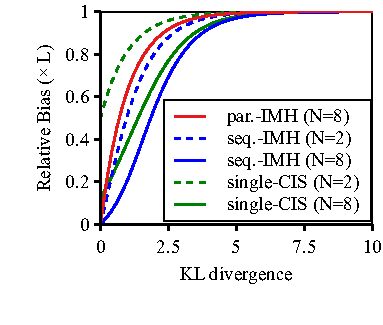
\includegraphics[scale=0.9]{figures/bias_01.pdf}
  \vspace{-0.35in}
  \caption{Relative bias of different estimators.
  For simplicity, we take \(w^* = \exp\left( \DKL{p}{q} \right)\).}\label{fig:bias}
\vspace{-0.1in}
\end{figure}
%
%% Since \(C_1\left(\vlambda\right) \rightarrow 0\) as \(\norm{\E{\vs\left(\vz; \vlambda\right)}} \rightarrow 0\), the bounds become tighter as SGD converges.
%% Furthermore, at the optimum, the bounds are deterministic regardless of \(\delta\).

\vspace{-0.05in}
\paragraph{Reducing Bias by Increasing \(N\)}
For the seq.-IMH estimator and single-CIS estimator, increasing \(N\) improves the bias decrease rate.
However, the bounds depend on \(w^*\), which is bounded below exponentially, as shown by the following proposition.
%
\begin{theoremEnd}{proposition}\label{thm:kl_bound}
  \(w^* = \sup_{\vz} \nicefrac{p\left(\vz\mid\vx\right)}{q_{\vlambda}\left(\vz\right)} \) is bounded below exponentially by the KL divergence such that
  \[
  \exp\left(\DKL{p\left(\cdot\mid\vx\right)}{ q_{\vlambda}\left(\cdot\right) }\right) \leq w^*.
  \]
\end{theoremEnd}
\vspace{-0.1in}
\begin{proofEnd}
  \begin{align*}
    &\DKL{p\left(\cdot\mid\vx\right)}{ q_{\vlambda}\left(\cdot\right) } \\
    &= \int p\left(\vz\mid\vx\right) \log \frac{p\left(\vz\mid\vx\right)}{q_{\vlambda}\left(\vz\right)}\,d\vz \\
    &\leq \int p\left(\vz\mid\vx\right) \log w^* \, d\vz \\
    &= \log w^*
  \end{align*}
\end{proofEnd}

Thus, in the initial steps of SGD, where the KL divergence is considerable, the bias will also be significant regardless of \(N\).
Therefore, increasing \(N\) will not bring a significant reduction in bias.
Also, since SGD achieves blinear convergence at best, under practical conditions, bias will be equally high on the the considered methods.
To illustrate this point, we visualized the bounds in~\cref{fig:bias}.


\begin{theoremEnd}{theorem}
  For a parallel state estimator with an IMH kernel, the bias is bounded as
  \[
  \mathrm{Bias}\left[ \vg_{\text{par.-IMH}} \right] \leq 
  C \, \sqrt{
    \chi^2\left( \pi \parallel q \right)
    +
    {\left(
      1 - \frac{1}{w^*}
      \right)}^2
  }
  \]
  where \(C = \Esub{p\left(\vz\mid\vx\right)}{\vs^2\left(\vz\right)}\), \(\chi^2\left(\pi \parallel q \right)\) is the Neyman Chi-square divergence, and \(w^* = \sup_{\vz} \nicefrac{\pi\left(\vz\right)}{q\left(\vz\right)} \).
\end{theoremEnd}
\begin{proofEnd}
  Let us denote \(\pi\left(\vz\right) = p\left(\vz\mid\vx\right)\) for conciseness.
  \begin{align}
    &\norm{
      \int K\left(\vz, \vz^*\right) \vs\left(\vz^*\right) d\vz^*
      - \int \pi\left(\vz\right) \vs\left(\vz\right) d\vz 
    }
    \\
    &=
    \norm{
      \int K\left(\vz, \vz^*\right) \vs\left(\vz^*\right) 
      - \pi\left(\vz^*\right) \vs\left(\vz^*\right) d\vz^*,
    }
    &\text{(\cref{thm:mh_ratio})}
    \\
    &=
    \norm{
      \int \pi\left(\vz^*\right) \min\left(\frac{1}{w\left(\vz\right)}, \frac{1}{w\left(\vz^*\right)}\right)  \vs\left(\vz^*\right) 
      - \pi\left(\vz^*\right) \vs\left(\vz^*\right) d\vz^*
    }
    \\
    &=
    \norm{
      \int \pi\left(\vz^*\right) \vs\left(\vz^*\right)
      \left(
      \min\left(\frac{1}{w\left(\vz\right)}, \frac{1}{w\left(\vz^*\right)}\right)  - 1  
      \right)
      d\vz^*
    }
    \\
    &=
    \sqrt{
      \Esub{\pi}{\vs^2}
    }
    \sqrt{
      \int \pi\left(\vz^*\right)
      {\left(
      \min\left(\frac{1}{w\left(\vz\right)}, \frac{1}{w\left(\vz^*\right)}\right)  - 1  
      \right)}^2
      d\vz^*.
    }
    &\text{(Cauchy-Schwarz)}
    \\
    \intertext{
     Now, let us denote \(A = \{\, \vz^* \mid w\left(\vz^*\right) > w\left(\vz\right) \,\}\).
     Then,
    }
    &=
    \sqrt{
      \Esub{\pi}{\vs^2}
    }
    \sqrt{
      \int_{A^c} \pi\left(\vz^*\right)
      {\left(
      \frac{1}{w\left(\vz^*\right)}  - 1  
      \right)}^2
      d\vz^*
      +
      \int_{A} \pi\left(\vz^*\right)
      {\left(
      \frac{1}{w\left(\vz\right)}  - 1  
      \right)}^2
      d\vz^*
    } \\
    &=
    \sqrt{
      \Esub{\pi}{\vs^2}
    }
    \sqrt{
      \int_{A^c} \pi\left(\vz^*\right)
      {\left(
      \frac{1}{w\left(\vz^*\right)}  - 1  
      \right)}^2
      d\vz^*
      +
      {\left(
      \frac{1}{w\left(\vz\right)}  - 1  
      \right)}^2
      \int_{A} \pi\left(\vz^*\right)
      d\vz^*
    }
    \\
    &\leq
    \sqrt{
      \Esub{\pi}{\vs^2}
    }
    \sqrt{
      \int_{A^c} \pi\left(\vz^*\right)
      {\left(
      \frac{1}{w\left(\vz^*\right)}  - 1  
      \right)}^2
      d\vz^*
      +
      {\left(
      \frac{1}{w\left(\vz\right)}  - 1  
      \right)}^2
    }
    \\
    &\leq
    \sqrt{
      \Esub{\pi}{\vs^2}
    }
    \sqrt{
      \int \pi\left(\vz^*\right)
      {\left(
      \frac{1}{w\left(\vz^*\right)}  - 1  
      \right)}^2
      d\vz^*
      +
      {\left(
      \frac{1}{w\left(\vz\right)}  - 1  
      \right)}^2
    }
    \\
    &=
    \sqrt{
      \Esub{\pi}{\vs^2}
    }
    \sqrt{
      \int \pi\left(\vz^*\right)
      {\left(
      \frac{q\left(\vz^*\right)}{\pi\left(\vz^*\right)}  - 1  
      \right)}^2
      d\vz^*
      +
      {\left(
      \frac{1}{w\left(\vz\right)}  - 1  
      \right)}^2
    }
    \\
    &\leq
    \sqrt{
      \Esub{\pi}{\vs^2}
    }
    \sqrt{
      \int \pi\left(\vz^*\right)
      {\left(
      \frac{q\left(\vz^*\right)}{\pi\left(\vz^*\right)}  - 1  
      \right)}^2
      d\vz^*
      +
      {\left(
      \frac{1}{w^*}  - 1  
      \right)}^2
    },
    \\
    \intertext{
      and finally, by the definition of the Neyman Chi-square divergence,
    }
    &=
    \sqrt{
      \Esub{\pi}{\vs^2}
    }
    \sqrt{
      \chi^2\left( \pi \parallel q \right)
      +
      {\left(
        1 - \frac{1}{w^*}
      \right)}^2
    }.
  \end{align}

  Lastly, for an arbitrary distribution \(\eta\left(\vz\right)\), 
  \begin{align}
    &\norm{
      \int \int \frac{1}{N} \sum^N_{i=1} \eta\left(\vz^{(i)}\right) K\left(\vz^{(i)}, \vz^*\right) \vs\left(\vz^*\right) \, d\vz^{(1:N)} \, d\vz^* - \Esub{\pi}{\vs}
    }
    &\text{(Independence of the chains)}
    \\
    &=
    \norm{
      \int \int \eta\left(\vz\right) K\left(\vz, \vz^*\right) \vs\left(\vz^*\right) d\vz \, d\vz^* - \Esub{\pi}{\vs}
    }
    &\text{(\cref{thm:kernel_apply_bias})}
    \\
    &\leq
    \sqrt{
      \Esub{\pi}{\vs^2}
    }
    \sqrt{
      \chi^2\left( \pi \parallel q \right)
      +
      {\left(
        1 - \frac{1}{w^*}
      \right)}^2
    }.
  \end{align}
\end{proofEnd}


%%% Local Variables:
%%% TeX-master: "master"
%%% End:


\vspace{-0.05in}
\subsection{Theoretical Analysis of Variance}
For MCMC estimators, variance often dominates the mean squared error.
Therefore, variance gives a better sense of their practical performance.

\vspace{-0.1in}
\paragraph{Variance of Single State Estimator}
The variance of the single estimator is given by the law of total variance such that
\vspace{-0.05in}
\begin{align}
  \V{\vg_{\text{single}}\left(\vlambda\right)} 
  &= \E{ \Vsub{K_{\vlambda_{t-1}}\left(\vz_{t-1}, \vz\right)}{ \vs\left(\vz; \vlambda\right) \mid \vz_{t-1} }} \nonumber \\
  &\quad + \V{ \Esub{K_{\vlambda_{t-1}}\left(\vz_{t-1}, \vz\right)}{ \vs\left(\vz; \vlambda\right) \mid \vz_{t-1} } }, \nonumber \\
  \intertext{and assuming stationarity such that \(\vz_{t-1} \sim p\left(\vz \mid \vx\right)\),}
  &= \Esub{p\left(\vz\mid\vx \right)}{ \Vsub{K_{\vlambda_{t-1}}\left(\vz_{t-1}, \vz\right)}{ \vs\left(\vz; \vlambda\right) \mid \vz_{t-1} }} \nonumber\\
  &\quad + \Vsub{p\left(\vz\mid\vx \right)}{ \Esub{K_{\vlambda_{t-1}}\left(\vz_{t-1}, \vz\right)}{ \vs\left(\vz; \vlambda\right) \mid \vz_{t-1} } } \nonumber \\
  &= \Vsub{p\left(\vz\mid\vx \right)}{\vs\left(\vz; \vlambda\right)} \nonumber \\
  &= \sigma^2.\nonumber
\end{align}
Ideally, the variance will be equal to the variance of an independent draw from the posterior.
This also suggests that, under stationarity, the variance of a single state estimator will be similar with any MCMC kernel.

\vspace{-0.05in}
\paragraph{Variance of Parallel State Estimator}
On the other hand, the parallel state estimator can be seen as an average of \textit{i.i.d.} single state estimators.
Therefore, under stationarity, the variance is
\vspace{-0.05in}
\begin{align*}
  \V{\vg_{\text{par.}}\left(\vlambda\right)} = \frac{\sigma^2}{N}
\end{align*}
\vspace{-0.05in}
Note that the variance reduction rate does not necessarily require stationarity.
The parallel state estimator thus \textit{always} enjoys \(\mathcal{O}\left(\nicefrac{1}{N}\right)\) variance reduction.

\vspace{-0.05in}
\paragraph{Variance of Sequential State Estimator}
Assuming stationarity, the variance of the sequential state estimator is given as
%
\vspace{0.05in}
{
\begin{align}
  &\V{\vg_{\text{seq.}}\left(\vlambda\right)} \nonumber\\
  &= \frac{\sigma^2}{N} + \frac{2}{N^2} \sum_{i < j}^N \Esub{p\left(\vz_T \mid \vx \right)}{ \Cov{ \vs\left(\vz_{i};\vlambda\right), \vs\left(\vz_{j};\vlambda\right) \mid \vz_{T} } }\label{eq:var_seq}.
\end{align}
}
which is similar to the variance of a regular MCMC estimator.
Here, \(T = N\,\left(t - 1\right)\) is the last state of the chain at the previous SGD iteration \(t-1\).
(Detailed derivation is in the \textit{supplementary material}.)
If the covariance term does not exist, the performance will be equal to the parallel state estimator.
However, due to rejections in the MCMC kernel, adjacent states will have some level of positive covariance.
Unfortunately, the rejection rate will be high when the KL divergence is significant, as implied by~\cref{thm:kl_bound}.
Thus, in practice, we can expect the performance of the sequential state estimator to be worse than the parallel state estimator.
This is the case as shown in the numerical simulation in~\cref{section:simulation}.

%
%
\begin{theoremEnd}[]{proposition}\label{thm:imh_bound}
  The rejection rate \(r\,(\vz_{t-1})\) of the IMH sampler is bounded below such that
  \[
  %r(\vz_{t-1}) \geq \frac{1}{1 + N\frac{q_{\vlambda}(\vz_{t-1})}{p(\vz_{t-1}\mid\vx)}}.
  r\,(\vz_{t-1}) \geq 1 - \nicefrac{Z}{w\,(\vz_{t-1})} 
  \]
  where \(Z=\int p\,(\vz,\vx) \, d\vz\) is the normalizing constant.
\end{theoremEnd}
\begin{proofEnd}
  The rejection rate \(r(\vz_{t-1})\) is given as
  \begin{align}
    r\,(\vz_{t-1}) = 1 - \int \alpha\left(\vz, \vz_{t-1} \right) \, q_{\vlambda}(\vz) \, d\vz.
  \end{align}
  For an IMH sampler with the Metropolis-Hastings acceptance function and independent proposals, the rejection rate is bounded such that
  \begin{align}
    r\,(\vz_{t-1})
    &= 1 - \int \min\left(\frac{w\,(\vz)}{w\,(\vz_{t-1})}, 1 \right) \, q_{\vlambda}(\vz)\,d\vz \\
    &= 1 - \frac{1}{w\,(\vz_{t-1})} \int \min\Big(w\,(\vz), w\,(\vz_{t-1})\Big) \, q_{\vlambda}(\vz)\,d\vz \\
    &= 1 - \frac{1}{w\,(\vz_{t-1})} \int \min\left(\frac{p\,(\vz,\vx)}{q_{\vlambda}(\vz)}, w\,(\vz_{t-1})\right) \, q_{\vlambda}(\vz)\,d\vz \\
    &=    1 - \frac{1}{w\,(\vz_{t-1})} \int \min\Big(p\,(\vz,\vx), w\,(\vz_{t-1})\,q_{\vlambda}(\vz)\Big) \, d\vz  \\
    &\geq 1 - \frac{1}{w\,(\vz_{t-1})} \int p\,(\vz,\vx) \, d\vz \label{eq:imh_min_comp} \\
    &=    1 - \frac{Z}{w\,(\vz_{t-1})} 
  \end{align}
  The inequality in Equation~\eqref{eq:imh_min_comp} follows from \(\min\big(p\,(\vz,\vx), w\,(\vz_{t-1})\,q_{\vlambda}(\vz)\big) \leq p\,(\vz,\vx) \) for \(\forall \vz \in \mathcal{Z}\).
\end{proofEnd}

%%% Local Variables:
%%% TeX-master: "master"
%%% End:

%

%
\begin{theoremEnd}{proposition}\label{thm:approx_var}
  Assuming \(w\,(\vz_{t-1})\) is large enough to make \(r\,(\vz\mid\vz^{(1:N)})\) independent of \(\vz^{(1:N)}\), the variance can be approximated by
  \begin{align}
    \Vsub{q_{\vlambda}}{ \E{ f \mid \vz_{t-1}, \vz^{(1:N)} } } \approx {\big(1 - r\,(\vz_{t-1})\big)}^2\,\Vsub{q_{\vlambda}}{ f_{\text{IS}} \,\middle\vert\, \vz_{t-1} }.
  \end{align}
\end{theoremEnd}
\begin{proofEnd}
  We evaluate the variance by approximating the rejection probability as an independent constant.
  First,
  \begin{align}
    &\Vsub{q_{\vlambda}}{ \E{ f \mid \vz_{t-1}, \vz^{(1:N)} } }. \\
    \intertext{
      Applying~\eqref{eq:cis_kernel_inter},
    }
    &= \Vsub{q_{\vlambda}}{ \big(1 - r\,(\vz_{t-1}\mid\vz^{(1:N)})\big)\, f_{\mathrm{IS}}
      + r\,(\vz_{t-1}\mid\vz^{(1:N)})\,f(\vz_{t-1}) \;\middle\vert\; \vz_{t-1}} \\
    &\approx \Vsub{q_{\vlambda}}{ \big(1 - r\,(\vz_{t-1})\big)\, f_{\mathrm{IS}}
      + r\,(\vz_{t-1})\,f(\vz_{t-1}) \;\middle\vert\; \vz_{t-1}} \\
    &= \Vsub{q_{\vlambda}}{ \big(1 - r\,(\vz_{t-1})\big)\, f_{\mathrm{IS}} \;\middle\vert\; \vz_{t-1} } \label{eq:approx_var_constant} \\
    &= {\big(1 - r\,(\vz_{t-1})\big)}^2 \, \Vsub{q_{\vlambda}}{ f_{\mathrm{IS}} \;\middle\vert\; \vz_{t-1} }. \label{eq:approx_var_linear} 
  \end{align}
  The equality of~\eqref{eq:approx_var_constant} follows from the fact that \(r\,(\vz_{t-1})\,f(\vz_{t-1})\) is a constant.
\end{proofEnd}

%%% Local Variables:
%%% TeX-master: "master"
%%% End:


%%% Local Variables:
%%% TeX-master: "master"
%%% End:
